\section{Persoalan Distribusi Kunci}
\label{sec:persoalan-distribusi-kunci}

Seluruh algoritma kunci-simetri yang telah dibahas --- DES, AES, RC5, dan GOST
--- memiliki satu syarat yang sama: pengirim dan penerima harus memegang kunci
rahasia yang identik. Syarat itu sederhana untuk diucapkan, tetapi menyimpan
persoalan yang jauh lebih sulit daripada rancangan algoritmanya sendiri. Bila
Alice ingin mengirim pesan terenkripsi kepada Bob, bagaimana ia menyampaikan
kunci itu kepada Bob tanpa kunci itu sendiri terbaca oleh pihak ketiga?

Pertanyaan itu dikenal sebagai \textbf{persoalan distribusi kunci}
(\textit{key distribution problem}). Sepanjang sejarah kriptografi modern ia
dijawab dengan cara yang sama: kunci diserahkan melalui saluran di luar sistem,
misalnya kurir yang dipercaya atau pertemuan tatap muka. Cara itu memang bekerja,
tetapi ongkosnya tumbuh jauh lebih cepat daripada jumlah penggunanya, dan
sebagaimana akan diperlihatkan, pertumbuhan itulah yang membuat persoalan ini
tidak dapat diabaikan.

\subsection{Pertumbuhan Jumlah Kunci yang Tidak Terkendali}

Pada Bab~\ref{chap:rsa} telah dihitung bahwa $n$ pengguna yang hanya memakai
kriptografi kunci-simetri memerlukan $\binom{n}{2} = n(n-1)/2$ kunci rahasia
berbeda, sebab setiap pasangan pengguna harus memiliki kunci tersendiri. Angka
itu tampak kecil untuk $n$ yang kecil: lima pengguna memerlukan sepuluh kunci.
Namun pertumbuhannya bersifat kuadratik, sehingga untuk organisasi berukuran
wajar pun hasilnya sudah tidak masuk akal:

\begin{itemize}
    \item 100 pengguna memerlukan 4.950 kunci;
    \item 1.000 pengguna memerlukan 499.500 kunci;
    \item 100.000 pengguna memerlukan 4.999.950.000 kunci --- hampir lima miliar
          kunci rahasia yang harus dibangkitkan, disimpan, dan dijaga.
\end{itemize}

Persoalannya bukan sekadar banyaknya berkas. Setiap kunci harus dibangkitkan
dengan keacakan yang baik, disimpan di tempat yang aman di kedua ujung, dan
diganti secara berkala. Bila satu kunci bocor, kerahasiaan satu pasangan
pengguna saja yang rusak --- keunggulan yang nyata dibandingkan kunci tunggal
yang dipakai bersama-sama --- tetapi beban pengelolaannya menjadi tidak praktis.

Kesulitan yang lebih mendasar muncul bahkan pada kasus paling sederhana, yaitu
dua pengguna. Untuk pertama kalinya, Alice dan Bob harus bertemu secara langsung
atau memakai kurir yang dipercaya agar dapat menyepakati kunci. Setelah kunci
itu ada, keduanya dapat berkomunikasi dengan aman; tetapi kunci itu harus
diganti secara berkala, dan setiap penggantian menuntut saluran rahasia yang
sama. Dengan kata lain, kriptografi kunci-simetri tidak menghapus kebutuhan akan
saluran rahasia sama sekali --- ia hanya memindahkannya dari seluruh isi
percakapan ke satu kunci pendek. Itu kemajuan yang besar, tetapi bukan
penyelesaian.

\subsection{Dua Jalan Keluar}

Ada dua cara keluar dari persoalan ini, dan keduanya dibandingkan pada
Tabel~\ref{tab:hibrida-vs-dh}.

\begin{enumerate}
    \item \textbf{Kriptografi hibrida} (\textit{hybrid cryptography}).
          Kunci rahasia tidak disepakati, melainkan \emph{dikirimkan}. Alice
          membangkitkan kunci sesi secara acak, lalu mengenkripsi kunci sesi itu
          dengan kunci publik Bob memakai RSA. Karena kunci sesi bersifat sangat
          pendek (misalnya 256 bit) sedangkan RSA hanya mampu menangani blok
          yang lebih pendek daripada modulusnya, cara ini justru memanfaatkan
          keterbatasan RSA sebagai kebaikan: yang dienkripsi dengan RSA hanyalah
          kunci, bukan pesannya. Cara ini dibahas pada
          Subbagian~\ref{subsec:hibrida-eksplisit}.
    \item \textbf{Protokol pertukaran kunci} (\textit{key exchange protocol}).
          Kunci rahasia tidak pernah dikirim sama sekali --- tidak dalam bentuk
          terang, tidak pula dalam bentuk terenkripsi. Kedua pihak justru
          \emph{menghitungnya sendiri} dari nilai-nilai yang dipertukarkan
          secara terbuka. Protokol Diffie--Hellman, yang menjadi pokok bahasan
          bab ini, adalah protokol pertukaran kunci yang pertama dan paling
          fundamental.
\end{enumerate}

\begin{table}[htbp]
    \centering
    \begin{tabular}{@{}>{\raggedright\arraybackslash}p{3.1cm}
                       >{\raggedright\arraybackslash}p{4.9cm}
                       >{\raggedright\arraybackslash}p{5.4cm}@{}}
    \toprule
    \textbf{Aspek} & \textbf{Kriptografi hibrida} & \textbf{Pertukaran kunci (DH)} \\
    \midrule
    Yang melewati saluran &
    Kunci sesi terenkripsi dengan RSA, beserta pesan terenkripsi &
    Hanya nilai publik $g^a$ dan $g^b$; tidak ada kunci yang melewati saluran \\
    \addlinespace
    Prasyarat &
    Kedua pihak telah memiliki kunci publik satu sama lain yang keasliannya
    terjamin &
    Kedua pihak menyepakati $p$ dan $g$; tidak diperlukan kunci publik
    perseorangan \\
    \addlinespace
    Ketergantungan pada kunci-publik &
    Ya, langsung: keamanan bergantung pada kerahasiaan kunci privat RSA &
    Tidak: DH dapat berdiri sendiri, tetapi tanpa otentikasi ia rapuh
    terhadap serangan aktif \\
    \addlinespace
    Sifat kunci yang dihasilkan &
    Dipilih oleh salah satu pihak, lalu dikirim &
    Dihitung bersama, tidak pernah ada di saluran \\
    \addlinespace
    Keunggulan menyusul &
    Dapat dipakai berkali-kali tanpa interaksi tambahan &
    Menghasilkan kunci baru setiap sesi sehingga memberi
    \textit{forward secrecy} \\
    \bottomrule
    \end{tabular}
    \caption{Perbandingan dua cara mengatasi persoalan distribusi kunci}
    \label{tab:hibrida-vs-dh}
\end{table}

Kedua cara itu tidak saling meniadakan. Protokol TLS yang mengamankan HTTPS
justru memakai keduanya sekaligus: Diffie--Hellman untuk menyepakati kunci sesi,
dan sertifikat berbasis kunci-publik untuk memastikan bahwa lawan bicaranya
benar-benar peladen yang dimaksud. Pemisahan peran itu penting: pertukaran kunci
memberi \emph{kerahasiaan}, sedangkan otentikasi memberi \emph{kepastian
identitas}, dan keduanya merupakan dua hal yang berbeda.

\subsection{Kriptografi Hibrida secara Terperinci}
\label{subsec:hibrida-eksplisit}

Langkah-langkah kriptografi hibrida diuraikan berikut ini secara lengkap.
Misalkan Alice ingin mengirim pesan $M$ kepada Bob, dan keduanya telah memiliki
pasangan kunci masing-masing: $(\text{SK}_{\text{Alice}}, \text{PK}_{\text{Alice}})$
dan $(\text{SK}_{\text{Bob}}, \text{PK}_{\text{Bob}})$.

\begin{enumerate}
    \item Alice membangkitkan kunci sesi $K$ secara acak dari
          pembangkit bilangan acak yang aman secara kriptografis. Kunci ini
          biasanya sepanjang 128 atau 256 bit, bergantung pada algoritma
          kunci-simetri yang dipakai.
    \item Alice mengenkripsi kunci sesi itu dengan kunci publik Bob memakai RSA:
          \[ E_{\text{RSA},\,\text{PK}_{\text{Bob}}}(K) = C_K . \]
          Hasilnya, $C_K$, adalah kunci sesi yang telah dibungkus. Panjangnya
          sama dengan panjang modulus RSA --- 256 byte untuk RSA-2048 --- jauh
          lebih panjang daripada kunci yang dibungkusnya.
    \item Alice mengenkripsi pesan $M$ dengan AES memakai kunci sesi $K$:
          \[ E_{\text{AES},\,K}(M) = C_M . \]
          Di sinilah letak efisiensinya: seluruh isi pesan diproses oleh AES,
          yang berjalan ratusan kali lebih cepat daripada RSA.
    \item Alice mengirimkan pasangan $(C_K, C_M)$ kepada Bob melalui saluran
          terbuka. Penyadap dapat membaca keduanya, tetapi tidak dapat
          memanfaatkannya.
    \item Bob mendekripsi $C_K$ dengan kunci privatnya sendiri:
          \[ D_{\text{RSA},\,\text{SK}_{\text{Bob}}}(C_K) = K . \]
          Hanya Bob yang dapat melakukan langkah ini, sebab hanya ia yang
          memegang $\text{SK}_{\text{Bob}}$.
    \item Bob mendekripsi pesan dengan kunci sesi yang baru saja diperolehnya:
          \[ D_{\text{AES},\,K}(C_M) = M . \]
\end{enumerate}

% Kriptografi hibrida: pesan yang melewati saluran dan pemulihannya di sisi Bob.
% Dirujuk dari section-01.tex dengan % Kriptografi hibrida: pesan yang melewati saluran dan pemulihannya di sisi Bob.
% Dirujuk dari section-01.tex dengan % Kriptografi hibrida: pesan yang melewati saluran dan pemulihannya di sisi Bob.
% Dirujuk dari section-01.tex dengan \input{figures/hibrida-pesan-dh}.
% Gambar diperkecil dengan \resizebox agar seluruh kotak muat dalam \linewidth.
\begin{figure}[htbp]
    \centering
    \resizebox{0.98\linewidth}{!}{%
    \begin{tikzpicture}[
        kotak/.style={draw, rounded corners=1pt, minimum height=0.95cm,
                      text width=2.9cm, align=center, font=\small, inner sep=3pt},
        panah/.style={-{Latex[length=2.2mm]}, thick},
        catatan/.style={font=\footnotesize, align=left, text width=13.6cm},
    ]
        % --- sisi Alice ---
        \node[kotak, fill=green!10] (kunci) at (0,0)
            {Kunci sesi $K$\\acak, 256 bit};
        \node[kotak, fill=orange!12] (aes) at (0,-2.3)
            {Pesan $M$};
        \node[kotak, fill=blue!6] (bungkus) at (3.8,0)
            {$C_K = E_{\mathrm{RSA},\mathrm{PK}_{\mathrm{Bob}}}(K)$};
        \node[kotak, fill=orange!12] (cm) at (3.8,-2.3)
            {$C_M = E_{\mathrm{AES},K}(M)$};

        \draw[panah] (kunci) -- (bungkus);
        \draw[panah] (aes) -- (cm);
        \draw[panah] (kunci) -- (aes);

        % --- saluran ---
        \node[kotak, fill=gray!12] (saluran) at (8.3,-1.15)
            {Saluran terbuka\\$C_K$ dan $C_M$};

        \draw[panah] (bungkus.east) -- (saluran.west);
        \draw[panah] (cm.east) -- (saluran.west);

        % --- sisi Bob ---
        \node[kotak, fill=blue!6] (buka) at (12.8,0)
            {$K = D_{\mathrm{RSA},\mathrm{SK}_{\mathrm{Bob}}}(C_K)$};
        \node[kotak, fill=green!10] (pulih) at (12.8,-2.3)
            {$M = D_{\mathrm{AES},K}(C_M)$};

        \draw[panah] (saluran.east) -- ++(0.5,0) -| (buka.north);
        \draw[panah] (saluran.east) -- ++(0.5,0) -| (pulih.north);
        \draw[panah] (buka) -- (pulih);

        \node[catatan, anchor=north] at (6.4,-3.4)
            {RSA menangani kunci sesi yang pendek, AES menangani seluruh isi
             pesan. Urutan pemulihan tidak dapat ditukar: $C_K$ memberi kunci,
             $C_M$ memberi isi};
    \end{tikzpicture}}
    \caption{Enam langkah kriptografi hibrida: $C_K$ dan $C_M$ melewati saluran
    terbuka, lalu dipertemukan kembali oleh Bob}
    \label{fig:hibrida-pesan-dh}
    \sumber{Munir, \textit{IF4020 Kriptografi}, ITB.}
\end{figure}
.
% Gambar diperkecil dengan \resizebox agar seluruh kotak muat dalam \linewidth.
\begin{figure}[htbp]
    \centering
    \resizebox{0.98\linewidth}{!}{%
    \begin{tikzpicture}[
        kotak/.style={draw, rounded corners=1pt, minimum height=0.95cm,
                      text width=2.9cm, align=center, font=\small, inner sep=3pt},
        panah/.style={-{Latex[length=2.2mm]}, thick},
        catatan/.style={font=\footnotesize, align=left, text width=13.6cm},
    ]
        % --- sisi Alice ---
        \node[kotak, fill=green!10] (kunci) at (0,0)
            {Kunci sesi $K$\\acak, 256 bit};
        \node[kotak, fill=orange!12] (aes) at (0,-2.3)
            {Pesan $M$};
        \node[kotak, fill=blue!6] (bungkus) at (3.8,0)
            {$C_K = E_{\mathrm{RSA},\mathrm{PK}_{\mathrm{Bob}}}(K)$};
        \node[kotak, fill=orange!12] (cm) at (3.8,-2.3)
            {$C_M = E_{\mathrm{AES},K}(M)$};

        \draw[panah] (kunci) -- (bungkus);
        \draw[panah] (aes) -- (cm);
        \draw[panah] (kunci) -- (aes);

        % --- saluran ---
        \node[kotak, fill=gray!12] (saluran) at (8.3,-1.15)
            {Saluran terbuka\\$C_K$ dan $C_M$};

        \draw[panah] (bungkus.east) -- (saluran.west);
        \draw[panah] (cm.east) -- (saluran.west);

        % --- sisi Bob ---
        \node[kotak, fill=blue!6] (buka) at (12.8,0)
            {$K = D_{\mathrm{RSA},\mathrm{SK}_{\mathrm{Bob}}}(C_K)$};
        \node[kotak, fill=green!10] (pulih) at (12.8,-2.3)
            {$M = D_{\mathrm{AES},K}(C_M)$};

        \draw[panah] (saluran.east) -- ++(0.5,0) -| (buka.north);
        \draw[panah] (saluran.east) -- ++(0.5,0) -| (pulih.north);
        \draw[panah] (buka) -- (pulih);

        \node[catatan, anchor=north] at (6.4,-3.4)
            {RSA menangani kunci sesi yang pendek, AES menangani seluruh isi
             pesan. Urutan pemulihan tidak dapat ditukar: $C_K$ memberi kunci,
             $C_M$ memberi isi};
    \end{tikzpicture}}
    \caption{Enam langkah kriptografi hibrida: $C_K$ dan $C_M$ melewati saluran
    terbuka, lalu dipertemukan kembali oleh Bob}
    \label{fig:hibrida-pesan-dh}
    \sumber{Munir, \textit{IF4020 Kriptografi}, ITB.}
\end{figure}
.
% Gambar diperkecil dengan \resizebox agar seluruh kotak muat dalam \linewidth.
\begin{figure}[htbp]
    \centering
    \resizebox{0.98\linewidth}{!}{%
    \begin{tikzpicture}[
        kotak/.style={draw, rounded corners=1pt, minimum height=0.95cm,
                      text width=2.9cm, align=center, font=\small, inner sep=3pt},
        panah/.style={-{Latex[length=2.2mm]}, thick},
        catatan/.style={font=\footnotesize, align=left, text width=13.6cm},
    ]
        % --- sisi Alice ---
        \node[kotak, fill=green!10] (kunci) at (0,0)
            {Kunci sesi $K$\\acak, 256 bit};
        \node[kotak, fill=orange!12] (aes) at (0,-2.3)
            {Pesan $M$};
        \node[kotak, fill=blue!6] (bungkus) at (3.8,0)
            {$C_K = E_{\mathrm{RSA},\mathrm{PK}_{\mathrm{Bob}}}(K)$};
        \node[kotak, fill=orange!12] (cm) at (3.8,-2.3)
            {$C_M = E_{\mathrm{AES},K}(M)$};

        \draw[panah] (kunci) -- (bungkus);
        \draw[panah] (aes) -- (cm);
        \draw[panah] (kunci) -- (aes);

        % --- saluran ---
        \node[kotak, fill=gray!12] (saluran) at (8.3,-1.15)
            {Saluran terbuka\\$C_K$ dan $C_M$};

        \draw[panah] (bungkus.east) -- (saluran.west);
        \draw[panah] (cm.east) -- (saluran.west);

        % --- sisi Bob ---
        \node[kotak, fill=blue!6] (buka) at (12.8,0)
            {$K = D_{\mathrm{RSA},\mathrm{SK}_{\mathrm{Bob}}}(C_K)$};
        \node[kotak, fill=green!10] (pulih) at (12.8,-2.3)
            {$M = D_{\mathrm{AES},K}(C_M)$};

        \draw[panah] (saluran.east) -- ++(0.5,0) -| (buka.north);
        \draw[panah] (saluran.east) -- ++(0.5,0) -| (pulih.north);
        \draw[panah] (buka) -- (pulih);

        \node[catatan, anchor=north] at (6.4,-3.4)
            {RSA menangani kunci sesi yang pendek, AES menangani seluruh isi
             pesan. Urutan pemulihan tidak dapat ditukar: $C_K$ memberi kunci,
             $C_M$ memberi isi};
    \end{tikzpicture}}
    \caption{Enam langkah kriptografi hibrida: $C_K$ dan $C_M$ melewati saluran
    terbuka, lalu dipertemukan kembali oleh Bob}
    \label{fig:hibrida-pesan-dh}
    \sumber{Munir, \textit{IF4020 Kriptografi}, ITB.}
\end{figure}


Perhatikan bahwa $C_K$ dan $C_M$ dikirim bersama-sama dan tidak bergantung satu
sama lain pada tingkat transmisi. Keduanya baru menjadi bermakna ketika
dipertemukan oleh Bob: $C_K$ memberi kunci, dan $C_M$ memberi isi. Karena itu
urutan pemulihan pada langkah 5 dan 6 tidak dapat ditukar.

Kunci sesi $K$ dibuang begitu sesi berakhir. Kebiasaan itu memberi keunggulan
yang tidak dimiliki pemakaian kunci statis: bila suatu saat kunci sesi lama
ternyata bocor, sesi-sesi yang sudah selesai tetap aman, sebab masing-masing
memakai kunci yang berbeda. Sifat ini akan muncul kembali dalam bentuk yang
lebih kuat pada pembahasan \textit{forward secrecy} di
Subbagian~\ref{subsec:forward-secrecy}.

\subsection{Analogi Pencampuran Cat}

Cara termudah memahami gagasan di balik pertukaran kunci Diffie--Hellman adalah
analogi pencampuran cat, yang diperlihatkan pada
Gambar~\ref{fig:analogi-cat-dh}. Alice dan Bob mula-mula menyepakati sebuah
warna yang tidak perlu dirahasiakan, misalnya kuning. Masing-masing kemudian
memilih warna rahasianya sendiri --- Alice memilih merah, Bob memilih biru. Alice
mencampur kuning dengan merah dan memperoleh jingga; Bob mencampur kuning dengan
biru dan memperoleh hijau muda. Keduanya bertukar hasil campuran itu melalui
kurir yang boleh jadi tidak dipercaya.

\begin{figure}[htbp]
    \centering
    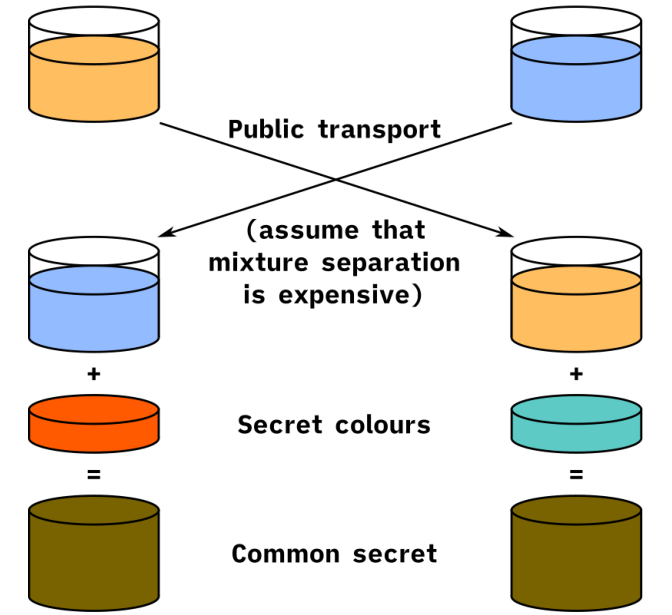
\includegraphics[width=0.78\linewidth, height=0.65\textheight, keepaspectratio]{figures/analogi-cat-dh.png}
    \caption{Analogi pencampuran warna cat: warna publik dipertukarkan secara
    terbuka, sedangkan warna rahasia masing-masing pihak menghasilkan campuran
    akhir yang identik}
    \label{fig:analogi-cat-dh}
    \sumber{Munir, \textit{IF4020 Kriptografi}, ITB.}
\end{figure}

Pada tahap terakhir, Alice mencampurkan warna rahasianya sendiri (merah) ke
campuran yang ia terima dari Bob (hijau muda), dan Bob mencampurkan warna
rahasianya (biru) ke campuran yang ia terima dari Alice (jingga). Keduanya kini
memegang warna yang sama, sebab pencampuran warna bersifat komutatif dan
asosiatif: merah dengan kuning dan biru menghasilkan hasil yang sama, tidak
peduli dalam urutan mana ketiganya dicampur.

Analogi ini memperlihatkan dua sifat yang menjadi inti protokol. Pertama,
pertukaran dilakukan pada nilai yang sudah tercampur sehingga penyadap tidak
dapat memisahkannya kembali. Kedua, hasil akhirnya sama di kedua sisi meskipun
keduanya menempuh urutan langkah yang berbeda.

Namun analogi ini juga menyesatkan pada satu hal, dan penting untuk menyadarinya.
Pada cat sungguhan, "memisahkan kembali" campuran adalah pekerjaan yang sulit
secara fisik karena pigmen benar-benar bercampur. Pada Diffie--Hellman, yang
sulit bukan pekerjaan fisik melainkan pekerjaan matematis: memulihkan $a$ dari
$g^a \bmod p$. Yang membuatnya sulit bukan ketiadaan cara, melainkan ketiadaan
cara yang cepat. Seorang penyerang dengan waktu tak terbatas selalu dapat
menemukan $a$ dengan mencoba seluruh kemungkinan; yang membuat protokol ini
berguna adalah kenyataan bahwa cara yang lebih cepat daripada itu belum
ditemukan sampai sekarang, dan bahwa rentang nilai $a$ dapat dibuat sangat besar.

Analogi itu juga tidak memperlihatkan kelemahan protokol ini. Sebagaimana
diuraikan pada Subbagian~\ref{subsec:mitm-dh}, seorang penyerang yang tidak hanya
menyadap melainkan juga ikut mencampur --- menukar warna yang dikirim dengan warna
buatannya sendiri --- dapat membuat Alice dan Bob masing-masing memegang warna
yang berbeda tanpa menyadarinya sama sekali.
